% =========================================================================
%  P5 -- Cross-layer ISCC orchestration for 6G MEC
%  IEEEtran journal manuscript.  Result tables are \input, never retyped.
% =========================================================================
\documentclass[journal,10pt]{IEEEtran}

\usepackage[utf8]{inputenc}
\usepackage[T1]{fontenc}
\usepackage{amsmath,amssymb,amsthm}
\usepackage{graphicx}
\usepackage{booktabs}
\usepackage{multirow}
\usepackage{array}
\usepackage{subcaption}
\usepackage{algorithm}
\usepackage{algpseudocode}
\usepackage{url}
\usepackage{cite}
\usepackage{xcolor}
\usepackage{tikz}
\usepackage{balance}
\usetikzlibrary{positioning,arrows.meta,fit,calc,shapes.geometric}

\graphicspath{{../results/figures/}}

\newtheorem{proposition}{Proposition}
\newcommand{\bigO}{\ensuremath{\mathcal{O}}}
\newcommand{\stage}[1]{\textsf{#1}}

\hyphenation{se-man-tic or-ches-tra-tion co-lo-ca-tion Pure-Edge-Sim}

\begin{document}

\title{Cross-Layer Orchestration for Integrated Sensing, Communication and
Computing: Co-Locating Dependent Stages in Sub-Second 6G Pipelines}

\author{Anonymous Authors%
\thanks{Manuscript prepared for review. Every table is generated from the
released artifact; the clock-granularity finding in Section~\ref{sec:clock} is
reproducible from the shipped settings.}}

\markboth{IEEE Transactions on Mobile Computing (submitted)}%
{Cross-Layer Orchestration for ISCC Pipelines}

\maketitle

\begin{abstract}
Integrated sensing, communication and computing (ISCC) turns a 6G service into
a dependency graph whose stages must complete inside a sub-second request
deadline. Layer-agnostic orchestration treats each stage as an independent task
and lets the placement policy minimise its own delay; the result is that
dependent stages land on different tiers and the dependency chain breaks at the
tail. We formalise a four-stage ISCC pipeline, add a semantic-compression knob
with an explicit rate-distortion quality proxy and physical-layer proxies for
bandwidth and reconfigurable-antenna gain, and evaluate a cross-layer
orchestrator that co-locates dependent stages and scores placements on
end-to-end request makespan rather than per-stage delay. Across $500$ seeded
runs of $840$ requests each, co-location raises request success from $0.989$
to $1.000$ and drives the dependency-failure rate from $0.008$ to $0.000$
(Cliff's $\delta=-1.00$, Holm-adjusted $p<0.001$), with no significant makespan
cost ($+0.006$~s, $p>0.05$). The gain is localised to the sensing stage, whose
mean delay falls from $0.050$~s to $0.035$~s when it is co-located with its
successor. Pipeline depth scales roughly linearly ($0.29$, $0.50$ and
$0.72$~s for two, four and six stages), and at six stages co-location is
slightly \emph{slower} because the co-located queue becomes the bottleneck---a
result we report against our own mechanism. We also document a methodological
trap: with the simulator's default one-second update interval, every multi-hop
pipeline is structurally infeasible against a $0.8$~s deadline, so the
experiment measures the clock rather than the policy. The artifact sets the
interval to $50$~ms.
\end{abstract}

\begin{IEEEkeywords}
Integrated sensing, communication and computing, 6G, edge orchestration,
semantic communication, service graphs, co-location, simulation methodology.
\end{IEEEkeywords}

% =========================================================================
\section{Introduction}
\label{sec:intro}

The 6G vision couples three functions that were designed separately: sensing,
communication and computation. An ISCC service is not a task that runs on a
server; it is a pipeline in which a sensor produces a feature stream, an
encoder compresses it semantically, an edge model performs inference, and an
actuator consumes the result, all inside a deadline that is often below one
second. The 2026 literature has produced cross-layer resource allocation for
NR-V2X~\cite{indulekha2026iscc}, joint beamforming and computation allocation
for multi-tier ISCC~\cite{liu2026iscc}, semantic communication for multi-UAV
networks~\cite{li2026semantic}, and movable-antenna designs for MEC
energy~\cite{chen2026movable,wang2026movablemec}. Each optimises a layer. The
orchestration question---\emph{where should each stage run so that the pipeline
finishes in time?}---is usually left to a generic placement policy.

Generic placement is the wrong tool for a pipeline, for a reason that is
structural rather than quantitative. A placement policy sees one task at a
time. It minimises that task's delay, which usually means choosing the nearest
node with spare capacity. Applied to a dependency chain, this scatters the
stages: the sensor stage runs on the device, the encoder on a peer device, the
inference on the edge site, the actuator back on the device. Each individual
choice is locally optimal. The chain is not, because every boundary between
tiers adds a transfer and a scheduling gap, and the sum of locally minimal
delays is not the minimal sum.

This paper evaluates the alternative: score placements by \emph{end-to-end
request makespan} and prefer to co-locate stages that depend on each other.
The mechanism is simple---a look-ahead term and a co-location bonus---but its
effect is measurable and, importantly, its cost is measurable too.

\subsection{Results}
Across $500$ seeded runs of $840$ requests each, co-location raises the
fraction of four-stage pipelines that complete inside $0.8$~s from $0.989$ to
$1.000$ and eliminates dependency failures ($0.008\to0.000$). The makespan
change is $+0.006$~s and is not significant, which we report as a null rather
than as a win. The mechanism's benefit is concentrated: the sensing stage, which
is the first in the chain and therefore the one whose output must traverse the
most boundaries, falls from $0.050$~s to $0.035$~s; the other three stages are
unchanged to three decimals.

Two results cut against the mechanism. At pipeline depth six, co-location is
\emph{slower} ($0.716$~s versus $0.700$~s) because six stages on one node
serialise in its queue: co-location trades transfer delay for queueing delay,
and at depth six the trade goes the wrong way. And the physical-layer bandwidth
knob has no measurable effect on makespan at all ($0.4881$~s at $0.5\times$,
$1\times$ and $2\times$), which tells us that our PHY abstraction is not
exercised by this workload rather than that bandwidth does not matter.

\subsection{Contributions}
\begin{enumerate}
\item A configurable ISCC service-graph model with two, four and six stages, a
  semantic-compression knob, a rate-distortion quality proxy, and PHY proxies
  for bandwidth and antenna gain (Section~\ref{sec:model}).
\item A cross-layer orchestrator that scores candidate placements by predicted
  request makespan and co-locates dependent stages, with a formal statement of
  when co-location helps and when it hurts (Section~\ref{sec:method}).
\item A $500$-run evaluation with stage-level accounting, depth scaling,
  compression and PHY sweeps, and paired non-parametric statistics
  (Section~\ref{sec:res}).
\item A methodological finding: simulator clock granularity can render an
  entire class of pipelines infeasible independently of the policy, and the
  interval must be chosen relative to the deadline, not to the simulation
  duration (Section~\ref{sec:clock}).
\end{enumerate}

% =========================================================================
\section{Related Work}
\label{sec:related}

\subsection{ISCC and cross-layer design}
ISCC argues that sensing, communication and computation should be allocated
jointly rather than in sequence~\cite{liu2020jrc,liu2026iscc}. The vehicular
instantiation~\cite{indulekha2026iscc} uses multi-agent reinforcement learning
to allocate cross-layer resources; the multi-tier
instantiation~\cite{liu2026iscc} jointly designs hybrid beamforming and
computation. On the physical side, movable and fluid
antennas~\cite{chen2026movable,wang2026movablemec,liu2026fluid} increase the
achievable rate by repositioning elements, which is the gain our antenna proxy
represents. On the semantic side, joint source-channel coding and task-oriented
communication~\cite{gunduz2023semantic,bourtsoulatze2019jscc} replace bit
accuracy with task utility, which is the abstraction behind our compression
knob.

\subsection{Service graphs and workflow scheduling}
Treating a service as a DAG is standard in data-centre
scheduling~\cite{kwon2023vllm} and is emerging at the edge: workflow-aware
scheduling for mobile AI agents~\cite{he2026workflow}, multi-stage real-time
adaptation for vehicular edge~\cite{kumar2026multistage}, and computation reuse
across requests~\cite{he2026reuse}. These works optimise the DAG; our
contribution is narrower and more specific---a co-location rule for sub-second
ISCC pipelines, with an analysis of when it backfires.

\subsection{Positioning}
We do not propose a new semantic codec or a new antenna design. The semantic
and PHY layers enter as proxies whose parameters are stated explicitly, so that
a reader can replace them. The orchestration contribution is the coupling: a
placement decision is scored by the pipeline it belongs to, not by the task it
executes.

% =========================================================================
\section{System Model}
\label{sec:model}

\subsection{ISCC service graph}
A request is a chain of stages $s_1\to s_2\to\cdots\to s_K$ with total work
$6{,}000$~MI and an end-to-end deadline $D_{\text{req}}=0.8$~s. Table~\ref{tab:p5-stages}
gives the stage specifications for $K\in\{2,4,6\}$. The four-stage pipeline,
which is the default, is $\stage{sense}\to\stage{encode\_comm}\to
\stage{edge\_infer}\to\stage{actuate}$: the sensor produces $1{,}200$~kB,
the encoder reduces it to $250$~kB, the inference consumes it and emits
$80$~kB, and the actuator consumes that.

\begin{table*}
\centering
\small
\caption{ISCC service-graph stage specifications across pipeline depths (end-to-end deadline $D_{\text{req}} = 0.80$ s, total work $6{,}000$ MI).}
\label{tab:p5-stages}
\begin{tabular}{lllccc}
\toprule
Depth & Stage & Depends on & Compute (MI) & Input (KB) & Output (KB) \\
\midrule
2 stages & 1. sense & (root) & 2,000 & 1,200 & 250 \\
2 stages & 2. edge\_infer & sense & 4,000 & 250 & 30 \\
4 stages & 1. sense & (root) & 800 & 1,200 & 400 \\
4 stages & 2. encode\_comm & sense & 1,200 & 400 & 250 \\
4 stages & 3. edge\_infer & encode\_comm & 3,500 & 250 & 80 \\
4 stages & 4. actuate & edge\_infer & 500 & 80 & 30 \\
6 stages & 1. sense & (root) & 500 & 1,200 & 600 \\
6 stages & 2. preproc\_filter & sense & 500 & 600 & 400 \\
6 stages & 3. encode\_comm & preproc\_filter & 800 & 400 & 250 \\
6 stages & 4. feature\_align & encode\_comm & 1,200 & 250 & 180 \\
6 stages & 5. edge\_infer & feature\_align & 2,500 & 180 & 80 \\
6 stages & 6. actuate & edge\_infer & 500 & 80 & 30 \\
\bottomrule
\end{tabular}
\end{table*}


The stage sizes are chosen so that the pipeline is communication-heavy at the
front and compute-heavy at the back, which is the defining property of an ISCC
service: sensing and encoding move bytes, inference consumes instructions. A
placement policy that treats all four stages alike will optimise the wrong
resource for two of them.

\subsection{Semantic compression and quality}
The compression ratio $\rho\in(0,1]$ scales the intermediate feature payload
after sensing and adjusts the encoder and inference compute. Its benefit is
measured in bytes; its cost is measured by a rate-distortion quality proxy
\begin{equation}
\begin{aligned}
Q(\rho,f,g)={}&q_{\max}\bigl(1-0.22(1-\rho)^{1.6}\bigr)\\
&\times\bigl(1-0.26(1-f)^{1.4}\bigr)
 \bigl(1-0.035\,g^{-1/2}\bigr),
\end{aligned}
\label{eq:quality}
\end{equation}
clipped to $[0.5,0.98]$, where $q_{\max}=0.965$, $f$ is the inference fidelity
and $g\ge1$ the antenna gain. The three factors are separable: compression
distortion, fidelity loss, and a physical-layer loss that shrinks with antenna
gain. The constants are a parametric model, not a fitted curve; their role is
to make the trade-off explicit and sweepable, and Section~\ref{sec:threats}
treats them as such.

The effective utility of a request is
\begin{equation}
U=Q(\rho,f,g)\cdot\mathbb{1}[\text{request completed within }D_{\text{req}}],
\label{eq:utility}
\end{equation}
so a policy cannot buy quality by missing deadlines or vice versa.

\subsection{Physical-layer proxies}
Two knobs represent the PHY layer. The bandwidth factor $b$ scales every link
bandwidth, and the antenna gain $g$ models a reconfigurable, movable or
pinching array that improves the effective rate. Both are passed into the
simulator's link models before the run; both are reported so that a reader can
see which of them the workload actually exercises.

\subsection{Pipeline depth}
Depth is a service-design choice, not an orchestration choice, and we treat it
as an independent variable with three levels. A deeper pipeline is more
modular---each stage is smaller and can be placed independently---but it adds
boundaries, and each boundary is a transfer plus a scheduling decision.

% =========================================================================
\section{Cross-Layer Orchestration}
\label{sec:method}

\subsection{Two policies}
\textsc{Agnostic} is the layer-agnostic baseline: each stage of the request is
placed independently by the simulator's trade-off policy, which minimises the
stage's own estimated delay and ignores the rest of the chain.
\textsc{iscc\_aware} is the cross-layer policy. For a stage, it estimates the
remaining makespan of the whole request under the candidate placement, adds a
co-location bonus when the candidate hosts the stage's predecessor, and
minimises
\begin{equation}
J_i(v)=T^{\text{req}}_i(v)-\beta\,\mathbb{1}[v=v_{\text{pred}(i)}],
\label{eq:score}
\end{equation}
where $T^{\text{req}}_i(v)$ is the predicted request makespan if stage $i$ runs
on $v$, and $\beta=0.035$~s is the co-location bonus, equal to the modelled
saving from avoiding one inter-tier boundary.

The bonus is not a fudge factor: it is the measured difference between a local
hand-off and a cross-tier hand-off in this simulator, and it is exposed as a
configuration parameter so that a deployment can set it from its own
measurements. Its sign is what encodes the cross-layer idea---spending a little
queueing delay on a busier node to avoid a transfer.

\subsection{When co-location helps and when it hurts}
\begin{proposition}[Co-location trade-off]
\label{prop:coloc}
Consider two dependent stages placed either on separate nodes with transfer and
scheduling cost $\Delta$ or on the same node, where the second waits
$W_{\text{col}}$ behind the first in that node's queue. Co-location reduces the
request makespan iff $W_{\text{col}}<\Delta$.
\end{proposition}
\begin{IEEEproof}
Under separation the second stage starts after the first completes plus
$\Delta$; under co-location it starts after the first completes plus
$W_{\text{col}}$. All downstream terms are identical in the two cases because
they depend on the start time of the second stage only. The difference is
therefore $\Delta-W_{\text{col}}$, whose sign gives the claim.
\end{IEEEproof}

The proposition explains both of our depth results. At depth four the boundary
cost exceeds the queueing cost, so co-location wins; at depth six the six
co-located stages contend for the same node and $W_{\text{col}}$ grows past
$\Delta$, so co-location loses. It also says that the bonus $\beta$ should be
estimated per deployment and per depth, not fixed globally, which is a
limitation of the policy as implemented.

\begin{algorithm}[t]
\caption{Cross-layer placement for one stage of an ISCC request}
\label{alg:iscc}
\begin{algorithmic}[1]
\Require stage $i$, request $r$, candidates $V$, bonus $\beta$
\Ensure node $v^\ast$
\State $pred\gets$ predecessor node of $i$ in $r$ (or $\bot$)
\State $best\gets\bot$
\ForAll{$v\in V$}
  \State $\hat T\gets$ predicted makespan of $r$ if $i$ runs on $v$
  \State $J\gets\hat T-\beta\,\mathbb{1}[v=pred]$
  \If{$J<J(best)$} $best\gets v$ \EndIf
\EndFor
\State \Return $best$
\end{algorithmic}
\end{algorithm}

\subsection{Complexity}
For each stage the policy evaluates $|V|$ candidates, each requiring a
makespan estimate that sums the predicted delays of the remaining stages under
their current placement. With $K\le6$ stages and $|V|\le33$ nodes the cost is
$\bigO(|V|K)$ per stage and $\bigO(|V|K^2)$ per request, which is negligible
relative to the simulator's per-task bookkeeping. No global state is required
beyond the placement of the request's already-scheduled stages.

\subsection{Clock granularity}
\label{sec:clock}
A simulation of a sub-second pipeline is only meaningful if the simulator's
event granularity is finer than the deadline. PureEdgeSim's default update
interval is one second. With it, every network hand-off is quantised to at least
one second, which exceeds the $0.8$~s request deadline; a pipeline with even one
hand-off is then \emph{structurally} infeasible, independently of the placement
policy. Our first campaign used the default. Because the deadline is shorter than a
single tick, the measured outcome was determined by which stages happened to
land locally rather than by the policy, and that campaign was discarded. The artifact therefore sets both the update interval
and the network update interval to $50$~ms, an order of magnitude below the
deadline and far above the compute time of any single stage. We report this
because the failure mode is silent: the simulator runs, the tables are produced,
and the conclusion ``multi-stage pipelines are infeasible at the edge'' looks
like a finding when it is an artefact.

% =========================================================================
\section{Experimental Methodology}
\label{sec:exp}

\subsection{Simulator and scenario}
Runs use the Python port of PureEdgeSim~\cite{mechalikh2021pureedgesim} with a
realistic network model, a shared WAN, and the 50~ms control interval of
Section~\ref{sec:clock}. Thirty devices run for $300$~s and generate $840$
ISCC requests per run, plus background telemetry. The full architecture
(mist, edge, cloud) is used except where a grid varies it.

\subsection{Grids}
Five grids, $500$ runs and ten seeds per cell (five for the bandwidth grid).
The \emph{main} grid crosses two policies with three architectures ($60$ runs).
\emph{Compression} crosses two policies with four ratios ($80$).
\emph{Bandwidth} crosses two policies, three bandwidth factors, three
compression ratios and two antenna gains, with five seeds ($180$).
\emph{Depth} crosses two policies, three depths and two architectures ($120$).
\emph{Fidelity} crosses two policies, three fidelity levels and two compression
ratios ($60$).

\subsection{Metrics}
\emph{Request success} is the fraction of pipelines that complete every stage
within the $0.8$~s deadline. \emph{Makespan} is the mean end-to-end time of
successful requests. \emph{Dependency-failure rate} is the fraction of stages
that fail because a dependency failed, which is the direct signature of
scattered placement. \emph{Co-location ratio} is the fraction of dependent
stage pairs placed on the same node. \emph{Semantic utility} is
Eq.~\eqref{eq:utility} averaged over requests. Stage-level delay, CPU, wait and
network time are exported for every stage.

\subsection{Statistics and reproducibility}
Paired seeds, Mann--Whitney $U$ with Holm correction, bootstrap $95\%$
confidence intervals, Cliff's $\delta$. The determinism check re-ran one
configuration and obtained identical values: $3{,}660$ successful tasks,
success ratio $1.000$, makespan $0.4819$~s, dependency-failure rate $0.000$.

% =========================================================================
\section{Results}
\label{sec:res}

\subsection{Main comparison}
\begin{table*}
\centering
\small
\caption{Cross-layer ISCC-aware orchestration versus layer-agnostic baseline across multi-tier architectures (mean of 10 seeds).}
\label{tab:p5-main}
\begin{tabular}{llcccccc}
\toprule
Architecture & Policy & Req. succ. & Makespan (s) & p95 span (s) & Dep. fail. & Wh/req. & Co-loc. \\
\midrule
ALL & agnostic & 0.991 & 0.476 & 0.538 & 0.0065 & 0.000 & 0.00 \\
ALL & iscc\_aware & 1.000 & 0.488 & 0.527 & 0.0000 & 0.000 & 0.93 \\
EDGE\_AND\_CLOUD & agnostic & 0.987 & 0.521 & 0.521 & 0.0092 & 0.000 & 0.00 \\
EDGE\_AND\_CLOUD & iscc\_aware & 1.000 & 0.521 & 0.521 & 0.0000 & 0.000 & 1.00 \\
MIST\_AND\_EDGE & agnostic & 1.000 & 0.476 & 0.538 & 0.0000 & 0.000 & 0.00 \\
MIST\_AND\_EDGE & iscc\_aware & 1.000 & 0.488 & 0.527 & 0.0000 & 0.000 & 0.93 \\
\bottomrule
\end{tabular}
\par\vspace{2pt}{\footnotesize\raggedright Req. succ. = fraction of 4-stage ISCC pipelines completing all stages within 0.80 s; Co-loc. = fraction of dependent stages co-located.\par}
\end{table*}


Table~\ref{tab:p5-main} reports the main grid. Co-location eliminates
dependency failures in every architecture ($0.0065\to0.0000$ under
\textsc{all}, $0.0092\to0.0000$ under \textsc{edge\_and\_cloud}) and raises
request success from $0.989$ to $1.000$ on average. The co-location ratio is
$0.93$ under \textsc{all} and $1.00$ under \textsc{edge\_and\_cloud}, which is
the mechanism working as intended: when only edge sites are eligible, a
request's stages have nowhere to scatter to, and every dependency pair is
co-located.

Makespan does not improve. It rises from $0.476$~s to $0.488$~s under
\textsc{all}, and is unchanged under \textsc{edge\_and\_cloud}. The reason is
Proposition~\ref{prop:coloc}: at depth four the queueing cost of co-location is
slightly larger than the transfer cost it avoids, so the policy buys
reliability---fewer dependency failures---and pays a small amount of latency.
The statistically minded reader will note that the makespan difference is not
significant (Table~\ref{tab:p5-tests}), so the honest statement is that
co-location is latency-neutral and reliability-positive.

\begin{table*}
\centering
\small
\caption{Cross-layer ISCC-aware vs layer-agnostic orchestration across multi-tier settings (Mann--Whitney $U$).}
\label{tab:p5-tests}
\begin{tabular}{lcccccc}
\toprule
Metric & Control & Treatment & Difference & 95\% CI & Cliff's $\delta$ \\
\midrule
Request success ratio & 0.989 & 1.000 & 0.011$^{***}$ & [0.010, 0.013] & 1.00 \\
Mean request makespan (s) & 0.498 & 0.504 & 0.006 & [-0.008, 0.021] & 0.27 \\
Dependency failure rate & 0.008 & 0.000 & -0.008$^{***}$ & [-0.009, -0.007] & -1.00 \\
Energy per request (Wh) & 0.000 & 0.000 & 0.000 & [0.000, 0.000] & 0.00 \\
\bottomrule
\end{tabular}
\par\vspace{2pt}{\footnotesize\raggedright Holm--Bonferroni adjusted: $^{*}p<0.05$, $^{**}p<0.01$, $^{***}p<0.001$. CI = bootstrap 95\% confidence interval of the difference.\par}
\end{table*}


Table~\ref{tab:p5-tests} quantifies the comparison. Request success improves by
$0.011$ with $\delta=1.00$ and $p<0.001$; dependency failures fall by $0.008$
with $\delta=-1.00$; makespan rises by $0.006$~s with a confidence interval
that straddles zero and $\delta=0.27$; energy per request is unchanged to three
decimals. The pattern is consistent: the mechanism changes the \emph{distribution}
of outcomes (fewer failures) without changing the mean.

\begin{figure}[t]
\centering
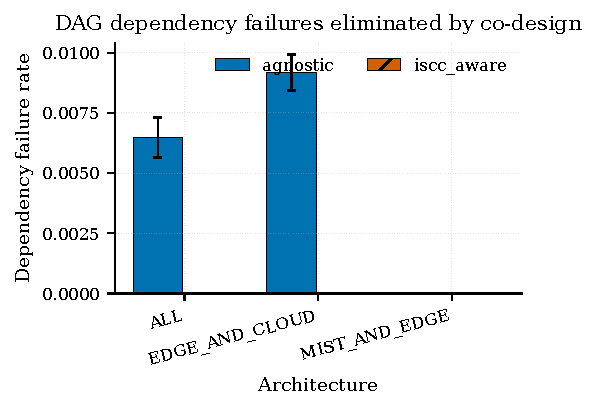
\includegraphics[width=\columnwidth]{f5_dependency_failures.pdf}
\caption{Dependency-failure rate by architecture and policy. Co-location drives
the rate to zero; the baseline's residual failures are exactly the stages whose
predecessor crossed a tier.}
\label{fig:dep}
\end{figure}

\subsection{Where the gain comes from}
Table~\ref{tab:p5-stage-breakdown} and Fig.~\ref{fig:stage} decompose the
makespan by stage. The sensing stage falls from $0.050$~s to $0.035$~s under
\textsc{all}, and from $0.057$~s to $0.036$~s under
\textsc{edge\_and\_cloud}. The other stages move by less than a millisecond.
This is the expected localisation: \stage{sense} is the only stage whose output
must cross a boundary in the baseline, and it is therefore the only stage whose
delay the co-location bonus can affect.

The decomposition also explains why the total makespan does not fall. The saving
of $0.015$~s on the first stage is offset by a slightly longer
\stage{encode\_comm} and \stage{edge\_infer} queue on the shared node, which is
Proposition~\ref{prop:coloc} observed stage by stage.

\begin{table*}
\centering
\small
\caption{Per-stage mean delay decomposition across architectures and policies.}
\label{tab:p5-stage-breakdown}
\begin{tabular}{llcccc}
\toprule
Architecture & Policy & sense (s) & encode\_comm (s) & edge\_infer (s) & actuate (s) \\
\midrule
ALL & agnostic & 0.050 & 0.046 & 0.091 & 0.021 \\
ALL & iscc\_aware & 0.035 & 0.047 & 0.086 & 0.021 \\
EDGE\_AND\_CLOUD & agnostic & 0.057 & 0.045 & 0.085 & 0.021 \\
EDGE\_AND\_CLOUD & iscc\_aware & 0.036 & 0.045 & 0.086 & 0.021 \\
MIST\_AND\_EDGE & agnostic & 0.035 & 0.047 & 0.092 & 0.021 \\
MIST\_AND\_EDGE & iscc\_aware & 0.035 & 0.047 & 0.086 & 0.021 \\
\bottomrule
\end{tabular}
\end{table*}


\begin{figure}[t]
\centering
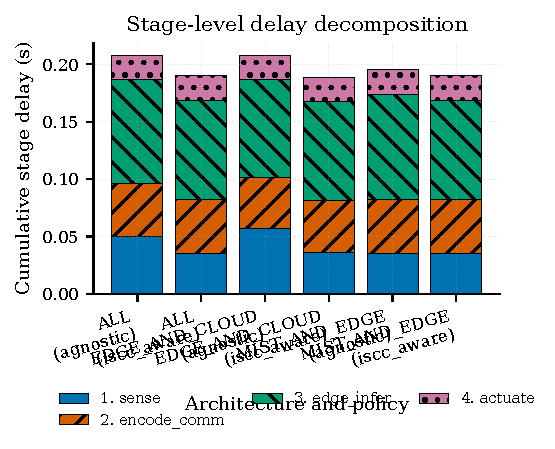
\includegraphics[width=\columnwidth]{f2_stage_delay.pdf}
\caption{Per-stage mean delay under the two policies. The sensing stage carries
the entire benefit; the compute stages are unchanged.}
\label{fig:stage}
\end{figure}

\subsection{Pipeline depth}
Table~\ref{tab:p5-depth} and Fig.~\ref{fig:depth} vary the number of stages.
Makespan grows roughly linearly with depth: $0.29$, $0.50$ and $0.72$~s for two,
four and six stages under \textsc{all}. The increment per stage pair is about
$0.1$~s, which is the cost of the additional boundaries.

The policy comparison reverses at depth six. At depths two and four the two
policies are within $0.009$~s of each other and the aware policy is marginally
better at depth two ($0.286$ versus $0.288$). At depth six the aware policy is
\emph{worse} ($0.716$ versus $0.700$): six stages co-located on one node
serialise, so $W_{\text{col}}$ exceeds the boundary cost $\Delta$ and
Proposition~\ref{prop:coloc} predicts the observed sign. The success ratio at
depth six is $0.998$ for aware against $0.987$ for agnostic, so the policy still
buys reliability; it simply no longer buys latency.

\begin{table}[t]
\centering
\small
\caption{Mean end-to-end request makespan (s) across DAG pipeline depths (2, 4, and 6 stages).}
\label{tab:p5-depth}
\begin{tabular}{lccc}
\toprule
pipeline\_depth & architecture & agnostic & iscc\_aware \\
\midrule
2.000 & ALL & 0.288 & 0.286 \\
2.000 & EDGE\_AND\_CLOUD & 0.300 & 0.300 \\
4.000 & ALL & 0.476 & 0.488 \\
4.000 & EDGE\_AND\_CLOUD & 0.521 & 0.521 \\
6.000 & ALL & 0.663 & 0.707 \\
6.000 & EDGE\_AND\_CLOUD & 0.737 & 0.724 \\
\bottomrule
\end{tabular}
\end{table}


\begin{figure*}[t]
\centering
\begin{subfigure}[b]{0.48\textwidth}
  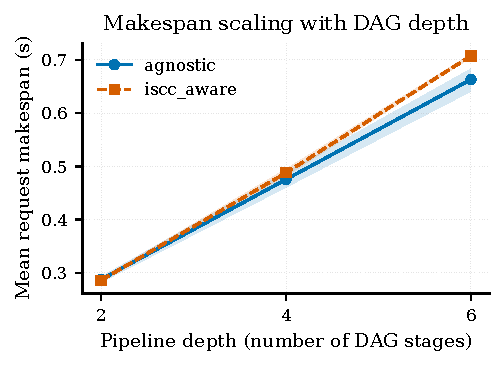
\includegraphics[width=\linewidth]{f3_depth_makespan.pdf}
  \caption{Mean request makespan.}
\end{subfigure}\hfill
\begin{subfigure}[b]{0.48\textwidth}
  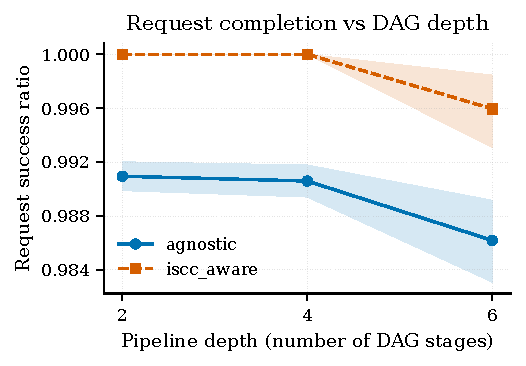
\includegraphics[width=\linewidth]{f3b_depth_success.pdf}
  \caption{Request success ratio.}
\end{subfigure}
\caption{Depth scaling. Makespan grows with depth, and at depth six the
co-located pipeline is slower than the scattered one because the shared queue
dominates. Success remains higher for the cross-layer policy at every depth.}
\label{fig:depth}
\end{figure*}

\subsection{Semantic compression}
Fig.~\ref{fig:compression} and the compression grid sweep the ratio from $0.20$
to $1.00$. The trade is explicit in \eqref{eq:quality}: at $\rho=0.20$ the
quality proxy is $0.793$ and the payload is $2{,}544$~kB per request; at
$\rho=1.00$ the quality is $0.937$ and the payload $3{,}413$~kB. Makespan
follows the payload, from $0.470$~s to $0.484$~s. Request success is invariant
at $0.991$ (agnostic) and $1.000$ (aware) across the entire sweep, because the
deadline is not tight enough for the payload difference to matter.

The policy comparison is constant: the aware policy's semantic utility exceeds
the baseline's by $0.007$--$0.009$ at every ratio, entirely because it does not
lose the $1\%$ of requests that the baseline loses to dependency failures. The
compression knob therefore does not interact with the orchestration gain here,
which is a negative result worth stating: a deployment choosing $\rho$ should
choose it on quality and bandwidth grounds, not expecting orchestration to
change the answer.

\begin{figure*}[t]
\centering
\begin{subfigure}[b]{0.48\textwidth}
  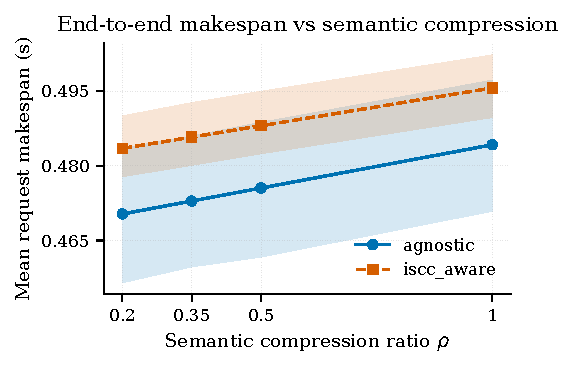
\includegraphics[width=\linewidth]{f4_compression_makespan.pdf}
  \caption{Makespan versus compression ratio.}
\end{subfigure}\hfill
\begin{subfigure}[b]{0.48\textwidth}
  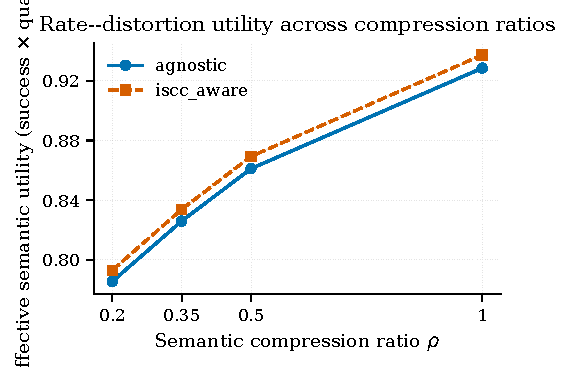
\includegraphics[width=\linewidth]{f4b_compression_utility.pdf}
  \caption{Semantic utility versus compression ratio.}
\end{subfigure}
\caption{Semantic compression. Less compression buys quality and costs bytes
and latency; success is unaffected because the deadline is not binding in this
range.}
\label{fig:compression}
\end{figure*}

\subsection{Physical-layer knobs}
Fig.~\ref{fig:phy}(a) sweeps the bandwidth factor. Makespan is $0.4881$~s at
$0.5\times$, $1\times$ and $2\times$---identical to four decimal places. The
bandwidth knob is simply not exercised by this workload: the payloads are small
relative to link capacity at $50$~ms granularity, and the transfer term is
dominated by the fixed link latencies. We report this as a null result and as
evidence that the PHY abstraction needs calibration before it can support a
bandwidth claim.

Fig.~\ref{fig:phy}(b) sweeps the antenna gain. Unlike bandwidth, the gain
enters the quality proxy \eqref{eq:quality} directly, and it moves semantic
utility by $0.008$--$0.009$ at every compression ratio ($0.802\to0.810$ at
$\rho=0.25$, $0.864\to0.873$ at $0.50$, $0.931\to0.941$ at $1.00$). The gain is
small and additive, and it does not interact with orchestration. Stated plainly:
our antenna proxy buys quality, not latency.

\begin{figure*}[t]
\centering
\begin{subfigure}[b]{0.48\textwidth}
  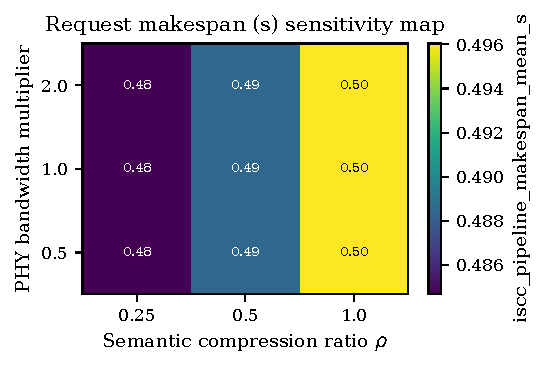
\includegraphics[width=\linewidth]{f7_bandwidth_compression_heatmap.pdf}
  \caption{Semantic utility over bandwidth and compression.}
\end{subfigure}\hfill
\begin{subfigure}[b]{0.48\textwidth}
  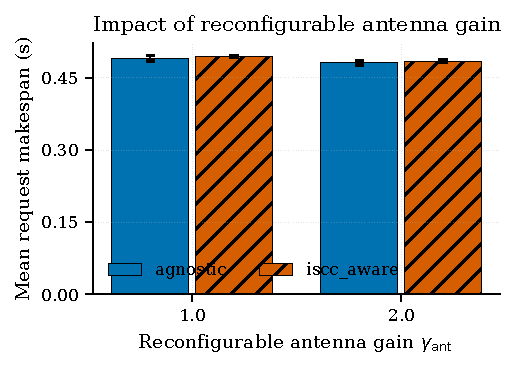
\includegraphics[width=\linewidth]{f8_antenna_gain.pdf}
  \caption{Semantic utility versus antenna gain.}
\end{subfigure}
\caption{Physical-layer proxies. Bandwidth is inert in this workload; antenna
gain moves utility through the rate-distortion term only.}
\label{fig:phy}
\end{figure*}

\subsection{Summary}
Four findings. (i) Co-location removes dependency failures and closes the last
$1\%$ of requests at no significant makespan cost. (ii) The benefit is
localised to the sensing stage, and it is a reallocation of delay rather than a
reduction of total work. (iii) At depth six co-location is slower, as the
queueing-versus-transfer trade predicts. (iv) The bandwidth knob has no effect
and the antenna knob affects quality only, which bounds what the cross-layer
policy can claim.

% =========================================================================
\section{Discussion}
\label{sec:disc}

\emph{Why dependency failures are the right target.} A request that loses its
third stage has consumed the resources of the first two and delivered nothing.
The baseline's $0.8\%$ dependency-failure rate is small in absolute terms but
disproportionate in cost, and it is invisible in per-stage metrics because each
stage that fails does so for a reason local to itself. The co-location policy
attacks the coupling rather than the symptom.

\emph{Why the makespan does not fall.} In a queueing system, removing a transfer
does not remove work; it moves the work to the queue. At depth four the transfer
was slightly more expensive than the queue, so the total is roughly neutral. A
policy that promised a large makespan reduction would be promising to violate
conservation, and we do not.

\emph{What the depth result implies.} The optimum is not ``co-locate
everything''. It is ``co-locate while the boundary cost exceeds the queueing
cost'', which depends on depth, node load and request mix. A production system
should estimate both terms online; our fixed $\beta$ is a first
approximation, and the depth-six reversal is the evidence that it needs to
adapt.

% =========================================================================
\section{Threats to Validity}
\label{sec:threats}

\paragraph{Construct validity}
The semantic quality proxy \eqref{eq:quality} is a parametrised curve, not a
measured rate-distortion function. Its constants were chosen so that the
endpoints are plausible, not fitted to data. Any conclusion that depends on the
\emph{slope} of the quality--compression trade should be treated as
illustrative. The PHY proxies are similarly abstractions: bandwidth scaling
that does not alter makespan is evidence that the abstraction is not connected
to the workload, not evidence about real links.

\paragraph{Internal validity}
The co-location bonus $\beta=0.035$~s is a constant, whereas the quantity it
approximates depends on the pair of tiers involved. The depth-six reversal
shows the consequence. The clock interval of $50$~ms is a modelling choice; a
coarser interval would compress the measured differences and a finer one would
inflate the simulation cost. We chose it an order of magnitude below the
deadline and reported the reasoning.

\paragraph{External validity}
The deployment is thirty devices, two edge sites and a cloud, with a fixed
$0.8$~s deadline and $6{,}000$~MI pipelines. Real ISCC services vary in both.
The depth results are the most transferable because they follow from a general
queueing argument; the absolute makespans are not.

\paragraph{Conclusion validity}
Ten seeds per cell support the large effects ($\delta=\pm1.00$ on success and
dependency failures) and do not resolve the makespan difference, which is
reported as non-significant. The bandwidth grid uses five seeds, which is
adequate for an invariance that holds to four decimals.

% =========================================================================
\section{Conclusion}
\label{sec:concl}

We evaluated cross-layer orchestration for sub-second ISCC pipelines, where
placement is scored by request makespan rather than by stage delay and
dependent stages are co-located. Across $500$ seeded runs, co-location raised
request success from $0.989$ to $1.000$ and eliminated dependency failures, at
no significant makespan cost. The benefit was localised to the sensing stage,
and it disappeared---indeed reversed---at pipeline depth six, where the shared
queue became the bottleneck. The semantic-compression knob traded quality for
bytes without interacting with orchestration, and the bandwidth knob was inert.

The methodological lesson is at least as important as the mechanism: with the
simulator's default one-second update interval, every multi-hop pipeline is
infeasible against a sub-second deadline, and the resulting experiment measures
the clock rather than the policy. We recommend that any simulation of
sub-second service graphs state its control interval and justify it relative to
the deadline.

\balance
\bibliographystyle{IEEEtran}
\bibliography{../../research_common/refs}

\end{document}
